%%%%%%%%%%%%%%%%%%%%%%%%%%%%%%%%%%%%%%%%%%%%%%%%%%%%%%%%%%%%%%%%%%%%%%%%%%%%%%%%%%%%%%%%%%%%%%%%%%%%%%
%
%   Filename    : chapter_5.tex 
%
%   Description : This file will contain your System Design.
%                 
%%%%%%%%%%%%%%%%%%%%%%%%%%%%%%%%%%%%%%%%%%%%%%%%%%%%%%%%%%%%%%%%%%%%%%%%%%%%%%%%%%%%%%%%%%%%%%%%%%%%%%

\chapter{FireflyX: Features and Design}

\section{System Overview}
FireflyX is a mobile application tool that aims to aid children in learning music fundamentals. There will only be one role, which is the user. The target users are children of ages 5 to 8 with varying knowledge in music. The user may edit the firefly models' parts based on their preferences.

The properties of the rhythm that can be configured on the firefly model are the tempo, length of the note, repetitions, rest pattern, and pitch. Each part of the firefly model directly corresponds to one property that can be modified.

The parts of the firefly model may be configured either by part or by manipulating the parts by gestures, such as dragging, swiping, and tapping. After a firefly model is configured, the user may set it free on a canvas where they can freely fly and roam. The rhythm will then be played with the properties set by the different parts the user has chosen or have tweaked. 

In order to create a rhythm, the user is allowed to make more firefly models with different configuration. The user will be allowed to play jar, load jars, preview, clear, edit previous firefly, and save their current jars.

\section{System Objectives}
The system aims to accomplish the following:
\begin{itemize}
    \item To enable users to make a rhythm and pitch using firefly models.
    \item To allow users to change the properties of the rhythm and pitch by tweaking the parts of the firefly model.
    \item To allow users to start playback by releasing the firefly models.
    \item To allow users to save and load their current jars.
\end{itemize}
\section{System Scope and Limitations}
The users can make rhythms by modifying the firefly models. We will only include rhythms and pitch, specifically claps and rests, no harmonies. The properties of the music can be modified by tweaking the parts of the firefly model.

The tempo of the firefly model can be chosen by the changing the body model. The body will be including only the 3 tempos used namely \textit{grave, adagio} and \textit{moderato}. The wing speed can be set by buttons to change the length of the note. The slower wing will represent slower notes and the faster wing will represent faster notes. For setting the repetition of the pattern, the wing size can be selected. The bigger sized wings will represent more repetitions, and the smaller sized wings will represent less repetitions. The speed and sizes will only be integers. The light of the firefly model is the pattern for the rests of the note. The number of patterns can be seen in Table \ref{Patterns}. Also the pitch will be represented by the candies scattered in the environment. 

Each workspace will be considered as a jar. The user is given five fireflies in jar to play with. After the user modifies the firefly models, they can be released outside the jar. Only five fireflies may roam outside freely, where the firefly will traverse through a trail which leads to it moving to another note's pitch. After the fireflies that are currently playing are finished, they will be automatically be saved as a track. The track will be added to the track list. The track will be represented also as a jar.

The users will be able to listen to previous tracks by loading them in the environment. The users are allowed to save their current workspace. The saved file will include the current album and the configurations of the fireflies. A JSON file format will be used for the saved files. These saved data can be loaded by the user at any time. Each save will ask the input for the title of the jar.

\section{Architectural Design}

\begin{figure} [H]
    \centering
    \includegraphics[width=15cm]{figures/NewSysArchi.png}
    \caption{The System Architecture of FireflyX}
    \label{fig:sysarchi}
\end{figure}

\begin{figure} [H]
    \centering
    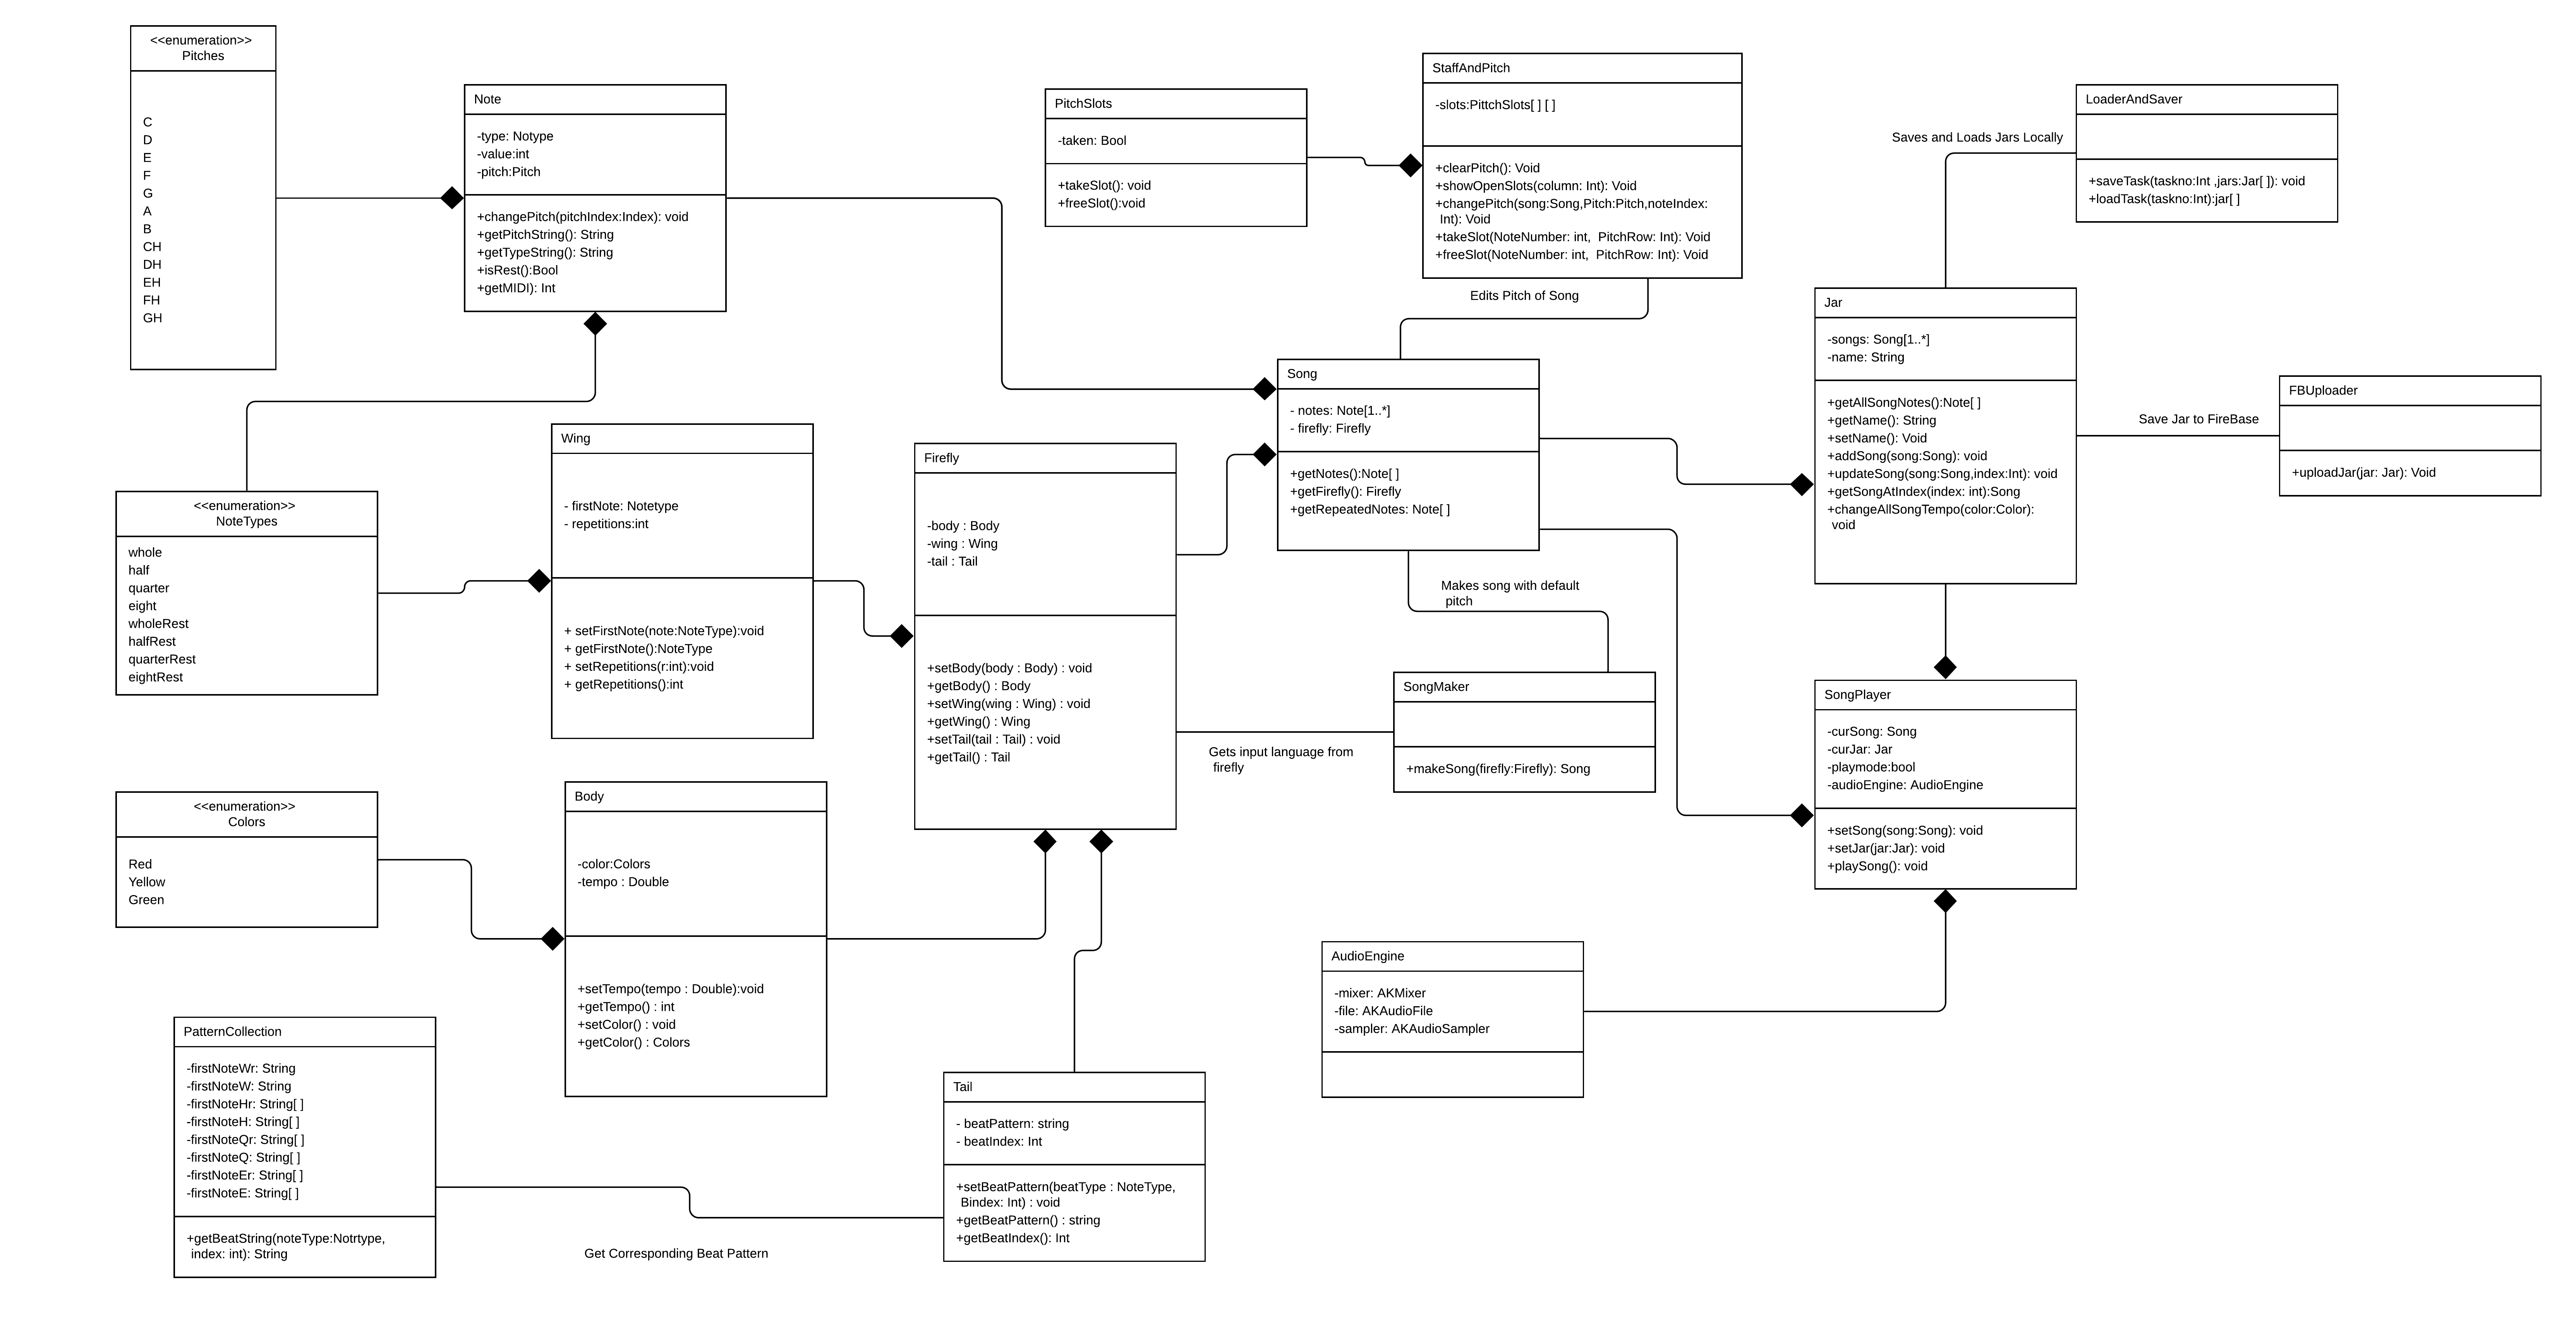
\includegraphics[width=17cm]{figures/NewFigure/FireflyXUML.png}
    \caption{UML class diagram of FireflyX}
    \label{fig:fireflyxUML}
\end{figure}

Figure \ref{fig:sysarchi} and Figure \ref{fig:fireflyxUML} shows the architecture of the system. The system follows a Model-View-Controller architecture. Most of the process will be handled locally by the device, but due to the pandemic we added a feature that saves their work on an online Database. Figure \ref{fig:fireflyxUML} shows the detailed class diagrams for the system.
    
\section{System Features}
The following are the features of the FireflyX application. Features such as firefly model parts popup settings, playback toolbox, jar sandbox environment, and the canvas.

% \subsection{Firefly Parts Toolbox}
% The toolbox serves to give the user the parts needed to make the firefly. The toolbox includes the head, body, wings, and the tails. Assembling different fireflies have different musical properties. These properties can be fine tuned using this toolbox. The chosen parts will correspond to a string of rhythm pattern language that will be parsed by our playback module when the firefly is released to the sandbox environment.

\subsubsection{Body Popup Settings}
The body section of the firefly model can be tapped to show the popup settings. In the popup settings of the body section, the user is able to choose the tempo of the firefly. Each unique color of the body has an equivalent tempo. The user can also scroll through a variety of body colors. The preferences of the body will be appended to the string of rhythm pattern language. For every environment once a body has been set for the first firefly the succeeding fireflies will have the same color with the first and by changing one the others get changed as well.

\subsubsection{Wings Popup Settings}
The wing section of the firefly model can be tapped to show the popup settings. In the popup settings of the wings section, the user is able to choose the speed of the note being played by pressing 1, 2, 4, and 8 which represents the whole note, half note, quarter note, eighth note, respectively or a picture of their notes itself. The size of the wing will represent the number of repetitions. The minimum size is 1 and the maximum size is 6. The wing preferences will be appended to the string of rhythm pattern language.

\subsubsection{Tail Light Popup Settings}
The tail section of the firefly model can be tapped to show the popup settings. On the right side, the user is able to change the rest pattern of the note being played. The tail lights will be representing the patterns and pattern can be previewed in a tail popup settings below, the light will be based from the chosen color in the body. The patterns will be predetermined by our library of patterns. The chosen pattern will be appended to the string of rhythm and pitch pattern language.

\subsubsection{Set Pitch Mode}
The mode is only accessible upon tapping the feed me button. The feed me button can be accessed during the tail pop settings. There will be a staff where the candies may be placed. The candies will be representing the notes. The number of candies will depend on the number of claps in the chosen pattern. The placement of the notes will also be determining the flight pattern of the firefly model. The preview button will also act like a playback for one specific firefly. The clear button will allow the user to reset the candies. The chosen pitch pattern will be appended to a separated pattern language.

\subsection{Jar Sandbox Environment}
The sandbox environment will be represented by a jar. In the jar, five firefly models can be seen where each can be tapped. When a firefly model is tapped, it enlarges and enables the popup settings when a specific part is tapped. The cork can also be tapped to release all of the firefly models into the canvas.

\subsection{Canvas}
Once the jar lid is tapped, the finished firefly models are released into the canvas where they roam around and play music based on their settings by sequence. Once the firefly models on the canvas are done playing they will be automatically be added to the list of jars.


\section{Music Language, Rules and Library of Patterns}

\begin{table}[H]
\caption{Rhythm representation}
\label{musiclang}
\centering
\begin{tabular}{|l|l|r|} 
\hline
note representation & music notation & integer equivalent  \\ 
\hline
W                   & Whole Note     & 1                   \\ 
\hline
H                   & Half Note      & 2                   \\ 
\hline
Q                   & Quarter Note   & 4                   \\ 
\hline
E                   & Eighth Note    & 8                   \\ 
\hline
Wr                  & Whole Rest     & -1                  \\ 
\hline
Hr                  & Half Rest      & -2                  \\ 
\hline
Qr                  & Quarter Rest   & -4                  \\ 
\hline
Er                  & Eighth Rest    & -8                  \\
\hline
\end{tabular}
\end{table}

\begin{table}[H]
\caption{Pitch representation}
\label{pitchVal}
\centering
\begin{tabular}{|l|l|r|} 
\hline
pitch of note & pitch representation   \\ 
\hline
c                   & (63)                     \\ 
\hline
d                   & (65)                      \\ 
\hline
e                   & (67)                      \\ 
\hline
f                   & (68)                    \\ 
\hline
g                   & (70)                      \\ 
\hline
a                   & (72)                       \\ 
\hline
b                   & (74)                    \\ 
\hline
c1                   & (75)                    \\ 
\hline
d1                   & (77)                    \\ 
\hline
e1                   & (79)                    \\ 
\hline
f1                   & (80)                    \\ 
\hline
g1                   & (82)                    \\ 
\hline
a1                   & (84)                    \\ 
\hline
Rest                   & (-)                    \\ 
\hline
\end{tabular}
\end{table}

\begin{table}[H]
\caption{Tempo representation}
\label{pitchRep}
\centering
\begin{tabular}{|l|l|r|} 
\hline
Name of Tempo & Beats Per Minute   \\ 
\hline
Grave                  & 25 bpm                     \\ 
\hline
Adagio                  & 60 bpm                      \\
\hline
Moderato                   & 100 bpm                       \\ 
\hline
\end{tabular}
\end{table}

To help us better understand the music sheets from the Book 1 of the Suzuki teaching method, we decided to convert the sheets to a language we can easily understand and represent on code. See Table \ref{musiclang} for reference to the converted language. This will mainly be used for the representation for the first iteration since at this iteration it only covers rhythm. To make the application easier to use, a set of rules for the music composition has been used. The firefly will only be using a maximum of 6 measures per rhythm. Each measure is equal to 1 pattern. The speed of the notes and rests that will be supported by the application will only be the whole, half, quarter, and eighth note.

The following patterns are taken from the Book 1 of the Suzuki teaching method, included here are the 3 most common clap and rest patterns found in each clap and rest combination (see Table \ref{Patterns}). For the representation in the table, 1 is for the clap and the 0 is for the rest. An example as seen from the table is "1Rest" - the number 1 coefficient represents the number of instances of the rest. A change in pattern from rest to tap is separated by a dash. 

For iteration two and three, since pitch will already be added we would use the same set of patterns and add a corresponding pitch (from C major scale) to a value in Swift audioKit denoted inside a parenthesis from the pitches found in Table \ref{pitchVal} and also how to represent ones from a rest. An example pattern is shown through part of two sample pieces of music (found in Appendix \ref{sec:appendixe}), the sample representation is seen in Table \ref{PitchPatterns}.

\begin{landscape}
\begin{table}
\centering
\caption{Common patterns in Suzuki Book 1}
\label{Patterns}
\begin{tabular}{|l|l|l|l|} 
\hline
 \textbf{Pattern}                                                                                                                                                              & \textbf{Pattern Name}                                                                                                                                                                                                    & \textbf{Count}                                                                                                                                                  & \textbf{Pattern Note Count}                                                                                                                                                                                                                \\ 
\hline
\begin{tabular}[c]{@{}l@{}}0 \\\\1\end{tabular}                                                                              & \begin{tabular}[c]{@{}l@{}}1Rest \\\\1Clap\end{tabular}                                                                                                                & \begin{tabular}[c]{@{}l@{}}23\\\\1\end{tabular}                                                               & \begin{tabular}[c]{@{}l@{}}{[}Wr - 23] \\\\{[}W - 1]\end{tabular}                                                                                                                        \\ 
\hline
\begin{tabular}[c]{@{}l@{}}001\\ \\ 010\\ \\ 100\end{tabular}              & \begin{tabular}[c]{@{}l@{}}2Rest-1Clap\\ \\ 1Rest-1Clap-1Rest\\ \\ 1Clap-2Rest \end{tabular}                         & \begin{tabular}[c]{@{}l@{}}12\\ \\ 6\\ \\ 2 \end{tabular}   & \begin{tabular}[c]{@{}l@{}}HrQrQ - 12]\\ \\ {[}QrQHr - 5, HrQQr - 1]\\ \\ {[}QQrHr - 2] \end{tabular}                                  \\ 
\hline
\begin{tabular}[c]{@{}l@{}}1010\\ \\ 1111\\ \\ 1110 \end{tabular}          & \begin{tabular}[c]{@{}l@{}}1Clap-1Rest-1Clap-1Rest\\ \\ 4Clap\\ \\ 3Clap-1Rest \end{tabular}                         & \begin{tabular}[c]{@{}l@{}}39\\ \\ 22\\ \\ 5 \end{tabular}  & \begin{tabular}[c]{@{}l@{}}QQrQQr - 39] \\ \\ {[}QQQQ - 21, EEQH - 1]\\ \\ {[}QQQQr - 5] \end{tabular}                                 \\ 
\hline
\begin{tabular}[c]{@{}l@{}}10110\\ \\ 11111\\ \\ 01101 \end{tabular}       & \begin{tabular}[c]{@{}l@{}}1Clap-1Rest-2Clap-1Rest\\ \\ 5Clap\\ \\ 1Rest-2Clap-1Rest-1Clap \end{tabular}             & \begin{tabular}[c]{@{}l@{}}26\\ \\ 10\\ \\ 13 \end{tabular} & \begin{tabular}[c]{@{}l@{}}QQrEEQr - 26]\\ \\ {[}QEEQQ -4, QQQEE -3, EQEQQ- 1, EEQQQ -1, EQQQE -1]\\ \\ {[}QrEEQrQ -13] \end{tabular}  \\ 
\hline
\begin{tabular}[c]{@{}l@{}}110110\\ \\ 111111\\ \\ 011011 \end{tabular}    & \begin{tabular}[c]{@{}l@{}}2Clap-1Rest-2Clap-1Rest\\ \\ 6Clap\\ \\ 1Rest-2Clap-1Rest-2Clap \end{tabular}             & \begin{tabular}[c]{@{}l@{}}20\\ \\ 3\\ \\ 6 \end{tabular}   & \begin{tabular}[c]{@{}l@{}} EEQrEEQr - 20 ]\\ \\ {[} EEQEEQ - 2, QQEQQE - 1 ]\\ \\ {[} QrEEQrEE - 6 ] \end{tabular}                    \\ 
\hline
\begin{tabular}[c]{@{}l@{}}1111111\\ \\ 0101011\\ \\ 0111011~\end{tabular} & \begin{tabular}[c]{@{}l@{}}7Clap\\ \\ 1Rest-1Clap-1Rest-1Clap-1Rest-2Clap\\ \\ 1Rest-3Clap-1Rest-2Clap \end{tabular} & \begin{tabular}[c]{@{}l@{}}14\\ \\ 4\\ \\ 2 \end{tabular}   & \begin{tabular}[c]{@{}l@{}} EEEEEEQ - 11, EEQEEEE - 3 ]\\ \\ {[} ErEErEErEQ - 4 ]\\ \\ {[} ErEEEErEQ - 2 ] \end{tabular}               \\ 
\hline
\begin{tabular}[c]{@{}l@{}}11110110\\ \\ 11111111 \end{tabular}                                                              & \begin{tabular}[c]{@{}l@{}}4Clap-1Rest-2Clap-1Rest\\ \\ 8Clap \end{tabular}                                                                                            & \begin{tabular}[c]{@{}l@{}}4\\ \\ 3 \end{tabular}                                                             & \begin{tabular}[c]{@{}l@{}}EEEEErEEEr - 4 ]\\ \\ {[}EEEEEEEE - 3 ] \end{tabular}                                                                                                         \\
\hline
\end{tabular}
\end{table}
\end{landscape}

\begin{table}
\centering
\caption{Some patterns found in Hot Cross Buns and Old Macdonald}
\label{PitchPatterns}
\begin{tabular}{|l|l|l|l|} 
\hline
 \textbf{Pattern }                                                                                     & \textbf{Pattern Name}                                                                                          & \textbf{Count}                                                                                   & \textbf{Pattern Note Count (with Pitch)}                                                                                                         \\ 
\hline
0                                                                                                      & 1Rest                                                                                                          & 1                                                                                                & {[}Wr(-) - 1]                                                                                                                                    \\ 
\hline
10                                                                                                     & 1Clap-1Rest                                                                                                    & 1                                                                                                & {[}H()Hr(-) - 1]                                                                                                                                \\ 
\hline
111                                                                                                    & 3Clap                                                                                                          & 3                                                                                                & {[}Q(b)Q(a)H(g) - 3]                                                                                                                             \\ 
\hline
\begin{tabular}[c]{@{}l@{}}1110\\\\1111\end{tabular} & \begin{tabular}[c]{@{}l@{}}3Clap-1Rest\\\\4Clap\end{tabular} & \begin{tabular}[c]{@{}l@{}}1\\\\1\end{tabular} & \begin{tabular}[c]{@{}l@{}}{[}Q(g)Q(g)Q(g)Qr(-) - 1]\\\\{[}Q(b)Q(b)Q(a)Q(a) - 1]\end{tabular}  \\ 
\hline
11111111                                                                                               & 8Clap                                                                                                          & 1                                                                                                & {[}E(b)E(b)E(b)E(b)E(a)E(a)E(a)E(a)]                                                                                                             \\
\hline
\end{tabular}
\end{table}

\section{Data Design}
Each selection of the firefly body part corresponds to an integer that references into a music library to get the necessary music files needed for the playback. The chosen format for the save files will be using JSON. The file will be saving all the configurations of the current fireflies on the canvas. The file can be loaded and it will load the fireflies with their configurations that were saved on the file. The saved files will be stored locally on the device. Allowed inputs for the files can be seen in the table below in Table 5.6. An example JSON file is also shown in Table \ref{XML} that shows how the sample piece Hot Cross Buns seen in Appendix \ref{sec:appendixe} will be saved.

% \begin{figure}[H]
%     \centering
%     \includegraphics[width=17.6cm]{figures/sampleXML.png}
%     \caption{Sample XML}
%     \label{sampleXML}
% \end{figure}

% \begin{landscape}
% \begin{table}
% \centering
% \caption{Data Design Specifics}
% \label{XML}
% \begin{tabular}{|l|} 
% \hline
% \begin{tabular}[c]{@{}l@{}}\textless{}album albumName = "Sample with Pitch" albumAuthor = "Ted"\textgreater{}	albAlbum1						\\~ ~ ~ ~ \textless{}track trackName = "Hot Cross Buns" \textgreater{}	trkTrack1					\\~ ~ ~ ~ ~ ~ ~ ~ \textless{}firefly fireflyName = "ffObj1"\textgreater{}					\\~ ~ ~ ~ ~ ~ ~ ~ ~ ~ ~ ~ \textless{}body color = "green" bpm = 60\textgreater{}	ffObj1Body			\\~ ~ ~ ~ ~ ~ ~ ~ ~ ~ ~ ~ ~ ~ ~ ~ \textless{}tail pattern = 111 count = 3 pitch = Q(b)Q(a)H(g)\textgreater{}	ffObj1Tail		\\~ ~ ~ ~ ~ ~ ~ ~ ~ ~ ~ ~ ~ ~ ~ ~ \textless{}/tail\textgreater{}			\\~ ~ ~ ~ ~ ~ ~ ~ ~ ~ ~ ~ \textless{}/body\textgreater{}				\\~ ~ ~ ~ ~ ~ ~ ~ ~ ~ ~ ~ \textless{}wings size = 2 speed = 4\textgreater{}	ffObj1Wings			\\~ ~ ~ ~ ~ ~ ~ ~ ~ ~ ~ ~ \textless{}/wings\textgreater{}\\~ ~ ~ ~ ~ ~ ~ ~ \textless{}/firefly\textgreater{}					\\~ ~ ~ ~ ~ ~ ~ ~ \textless{}firefly fireflyName = "ffObj2"\textgreater{}					\\~ ~ ~ ~ ~ ~ ~ ~ ~ ~ ~ ~ \textless{}body color = "green" bpm = 60\textgreater{}	ffObj2Body			\\~ ~ ~ ~ ~ ~ ~ ~ ~ ~ ~ ~ ~ ~ ~ ~ \textless{}tail pattern = 11111111 count = 8 pitch = E(b)E(b)E(b)E(b)E(a)E(a)E(a)E(a)\textgreater{}	ffObj2Tail		\\~ ~ ~ ~ ~ ~ ~ ~ ~ ~ ~ ~ ~ ~ ~ ~ \textless{}/tail\textgreater{}			\\~ ~ ~ ~ ~ ~ ~ ~ ~ ~ ~ ~ \textless{}/body\textgreater{}				\\~ ~ ~ ~ ~ ~ ~ ~ ~ ~ ~ ~ \textless{}wings size = 1 speed = 8\textgreater{}	ffObj2Wings			\\~ ~ ~ ~ ~ ~ ~ ~ ~ ~ ~ ~ \textless{}/wings\textgreater{}\\~ ~ ~ ~ ~ ~ ~ ~ ~\textless{}/firefly\textgreater{}					\\~ ~ ~ ~ ~ ~ ~ ~ ~\textless{}firefly fireflyName = "ffObj3"\textgreater{}					\\~ ~ ~ ~ ~ ~ ~ ~ ~ ~ ~ ~ \textless{}body color = "green" bpm = 60\textgreater{}	ffObj3Body			\\~ ~ ~ ~ ~ ~ ~ ~ ~ ~ ~ ~ ~ ~ ~ ~ \textless{}tail pattern = 111 count = 3 pitch = Q(b)Q(a)H(g)\textgreater{}	ffObj3Tail		\\~ ~ ~ ~ ~ ~ ~ ~ ~ ~ ~ ~ ~ ~ ~ ~ \textless{}/tail\textgreater{}			\\~ ~ ~ ~ ~ ~ ~ ~ ~ ~ ~ ~ \textless{}/body\textgreater{}				\\~ ~ ~ ~ ~ ~ ~ ~ ~ ~ ~ ~ \textless{}wings size = 1 speed = 4\textgreater{}	ffObj3Wings~ \\~ ~ ~ ~ ~ ~ ~ ~ ~ ~ ~ ~ \textless{}/wings\textgreater{}\\~ ~ ~ ~ ~ ~ ~ ~ \textless{}/firefly\textgreater{}	\\~ ~ ~ ~ \textless{}/trackName\textgreater{}						\\\textless{}/album\textgreater{}	\end{tabular}  \\
% \hline
% \end{tabular}
% \end{table}
% \end{landscape}

\begin{table}
\centering
\caption{JSON data design}
\label{XML}
\begin{tabular}{|l|} 
\hline
\begin{tabular}[c]{@{}l@{}}jarObject~: \{\\~ ~ ~ ~ {}"JarName" : "Hot Cross Buns",\\\ ~ ~ ~ ~{}"Tempo" : 60,\\\ ~ ~ ~ ~"Fireflies" : \{\\~ ~ ~ ~ ~ ~ ~ ~"Firefly1" : \{\\ ~ ~ ~ ~ ~ ~ ~ ~ ~ ~ ~ ~"Beat Pattern" : "Q Q H",\\~ ~ ~ ~ ~ ~ ~ ~ ~ ~ ~ ~"Pitch Pattern" : "b a g",\\ ~ ~ ~ ~ ~ ~ ~ ~ ~ ~ ~ ~"Repetitions" : 2\\~ ~ ~ ~ ~ ~ ~ ~\},\\~ ~ ~ ~ ~ ~ ~ ~"Firefly2" : \{\\~ ~ ~ ~ ~ ~ ~ ~ ~ ~ ~ ~"Beat Pattern" : "E E E E E E E E",\\~ ~ ~ ~ ~ ~ ~ ~ ~ ~ ~ ~"Pitch Pattern" : "b b b b a a a a",\\~ ~ ~ ~ ~ ~ ~ ~ ~ ~ ~ ~"Repetitions" : 1\\~ ~ ~ ~ ~ ~ ~ ~\},\\~ ~ ~ ~ ~ ~ ~ ~"Firefly3" : \{\\~ ~ ~ ~ ~ ~ ~ ~ ~ ~ ~ ~"Beat Pattern" : "Q Q H",\\~ ~ ~ ~ ~ ~ ~ ~ ~ ~ ~ ~"Pitch Pattern" : "b a g",\\~ ~ ~ ~ ~ ~ ~ ~ ~ ~ ~ ~"Repetitions" : 1\\~ ~ ~ ~ ~ ~ ~ ~\}\\~ ~ ~ ~\}\\\}\end{tabular}  \\
\hline
\end{tabular}
\end{table}

% \begin{landscape}
% \begin{table}[]
% \label{XML}
% \caption{Data Design Specifics}
% \begin{tabular}{|l|l|l|l|}
% \hline
% Tags                            & Possible inputs              & Description                                                                                                                                                               & Correspondence \\ \hline
% \textless{}album\textgreater{}       & varchar     & \begin{tabular}[c]{@{}l@{}}The album will contain the author, \\ \\ album name, and tracks.\end{tabular}                                                                  & 1-*            \\ \hline
% \textless{}track\textgreater{}       & fireflies                    & \begin{tabular}[c]{@{}l@{}}There will be a maximum of 5 fireflies per\\ track.\end{tabular}                                                                               & 1-*            \\ \hline
% \textless{}firefly\textgreater{}     & body, wings, and tail light  & \begin{tabular}[c]{@{}l@{}}The firefly represents a rhythm that the\\ user defined by assembling their firefly.\end{tabular}                                              & 1-*            \\ \hline
% \textless{}body\textgreater{}        & sequence and instrument      & \begin{tabular}[c]{@{}l@{}}The body represents the sequence and\\ instrument of the rhythm.\end{tabular}                                                                  & 1-*            \\ \hline
% \textless{}sequence\textgreater{}    & 1,2,3,4,5                    & \begin{tabular}[c]{@{}l@{}}Represents the order of playback in the canvas. \\ \\ 1 means its the first firefly to run, 3, means 3rd.\end{tabular}                         & 1-1            \\ \hline
% \textless{}instrument\textgreater{}  & Guitar, Piano, Violin, Drum, & Represents the instrument to be played back.                                                                                                                              & 1-1            \\ \hline
% \textless{}wings\textgreater{}       & speed and size               & \begin{tabular}[c]{@{}l@{}}The wings represent the speed\\ and repetitions of the rhythm.\end{tabular}                                                                    & 1-*            \\ \hline
% \textless{}speed\textgreater{}       & 1,2,4,8                      & \begin{tabular}[c]{@{}l@{}}Represents the seed of the note. 1 means\\ \\ whole note, 2 means half note, \\ \\ 4 means quarter note, and 8 means eighth note.\end{tabular} & 1-1            \\ \hline
% \textless{}size\textgreater{}        & 1,2,3,4,5,6                  & \begin{tabular}[c]{@{}l@{}}Represents the number\\ of repetition of the firefly.\end{tabular}                                                                             & 1-1            \\ \hline
% \textless{}taillight\textgreater{}   & Rest pattern and color       & \begin{tabular}[c]{@{}l@{}}Represents the rest pattern and color\\ of the rhythm.\end{tabular}                                                                            & 1-*            \\ \hline
% \textless{}restpattern\textgreater{} & Check library of patterns    & \begin{tabular}[c]{@{}l@{}}Represents the clap rest\\ pattern of the firefly. Example is \\ 1010 which means clap - rest - clap - rest\end{tabular}                       & 1-1            \\ \hline
% \textless{}color\textgreater{}       & Hex-code of colors            & \begin{tabular}[c]{@{}l@{}}Represents the color emitted by the tail light of\\ the firefly. Example is \#FFFFFF means white.\end{tabular}                                 & 1-1            \\ \hline
% \end{tabular}
% \end{table}
% \end{landscape}

\begin{landscape}
\begin{table}
\centering
\caption{JSON data design specifics}
\label{XML}
\begin{tabular}{|p{2.8cm}|p{6.6cm}|p{9cm}|} 
\hline
\textbf{Variables} & \textbf{Possible Values}  & \textbf{Description}                                                                                                                                                                                                                    \\ 
\hline
JarName~~          & string~                   & This contains the album name that is specified by the user.                                                                                                                                                                             \\ 
\hline
Tempo              & integer~                  & It represents the tempo of the firefly, the colors are limited to the three colors imitating stoplights which are red,yellow, and green.                                                                                                \\ 
\hline
Fireflies          & array~                    & This contains the array of fireflies that are configured by the user which has a maximum of 5 fireflies per jar. Inside the array are the configured beat pattern, pitch pattern, and number of repetitions that was made by the user.  \\ 
\hline
Beat Pattern       & string                    & This contains the beat-rest pattern. For example a beat of QQQQ which is a 4Clap pattern with a count of 4.                                                                                                                             \\ 
\hline
Pitch Pattern      & string                    & This contains the pitch pattern which is retrieved from the making of the candies that represent the different pitches.                                                                                                                 \\ 
\hline
Repetition         & integer                   & This represents the configured right wing which is the number of times or repetitions the firefly will play once released to the environment.                                                                                           \\
\hline
\end{tabular}
\end{table}
\end{landscape}

\section{Screen Flows}
\label{sec: it3results}

% All use cases can be seen in Appendix \ref{sec:appendixb}.

\subsection{Splash Screen}

\begin{figure}[H]
    \centering
    
\includegraphics[width=10cm]{figures/newScreenFlows/newSplash.png}
    \caption{Splash screen}
    \label{fig:splash}
\end{figure}

The Splash Screen is the first screen shown to the child when the application is opened. The splash screen will last for 3 seconds.

\subsection{Home Screen}

\begin{figure}[H]
    \centering
    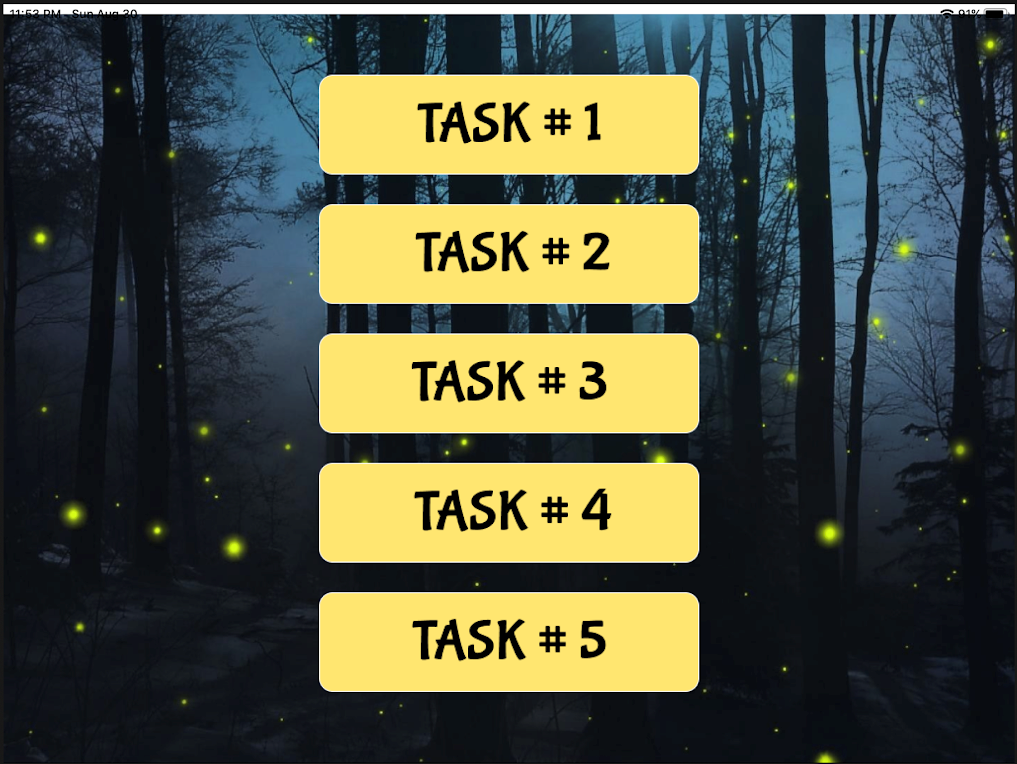
\includegraphics[width=10cm]{figures/newScreenFlows/newMain.png}
    \caption{Home screen}
    \label{fig:newhome}
\end{figure}

The Home Screen (figure \ref{fig:newhome}) is the next screen that will show after the splash screen, here the child may tap between 5 buttons, namely: Task \#1, Task \#2, Task \#3 ,Task \#4 ,and Task \#5. This is where the child will be doing the tasks for testing.

\subsection{First Firefly Screen}

\begin{figure}[H]
    \centering
    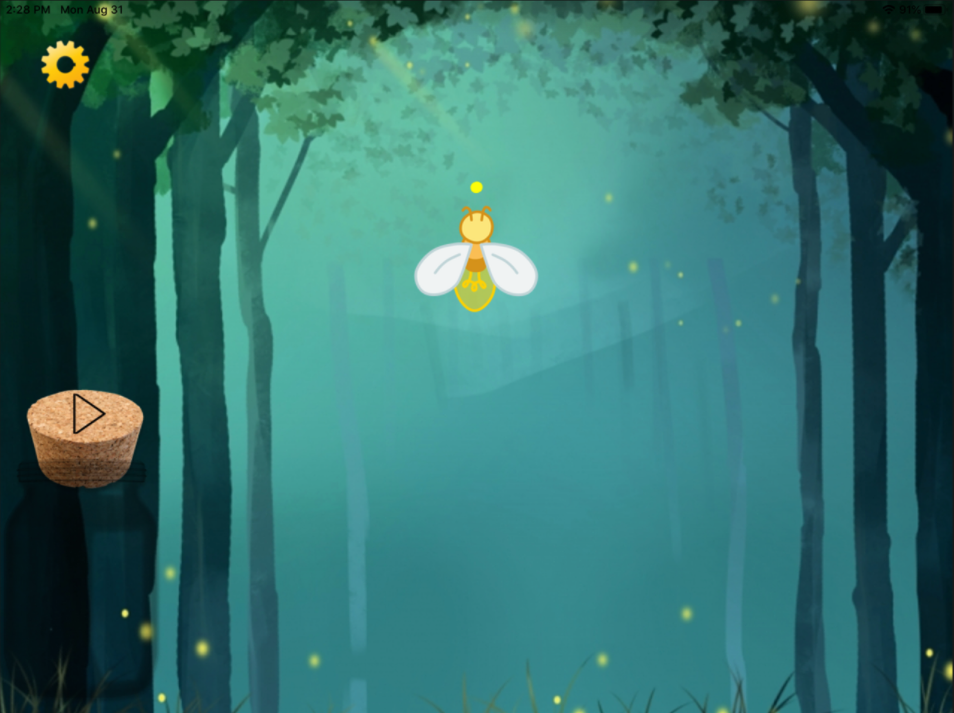
\includegraphics[width=5cm]{figures/newScreenFlows/newfirstfirefly.png}
    \caption{First firefly}
    \label{fig:firstfly}
\end{figure}

After going in to a task, the child will be greeted by a forest environment and a single firefly.
This will be the first firefly that the child can play around with and tweak to their heart's content.

\subsection{Firefly Body Selection}

\begin{figure}[H]
    \centering
    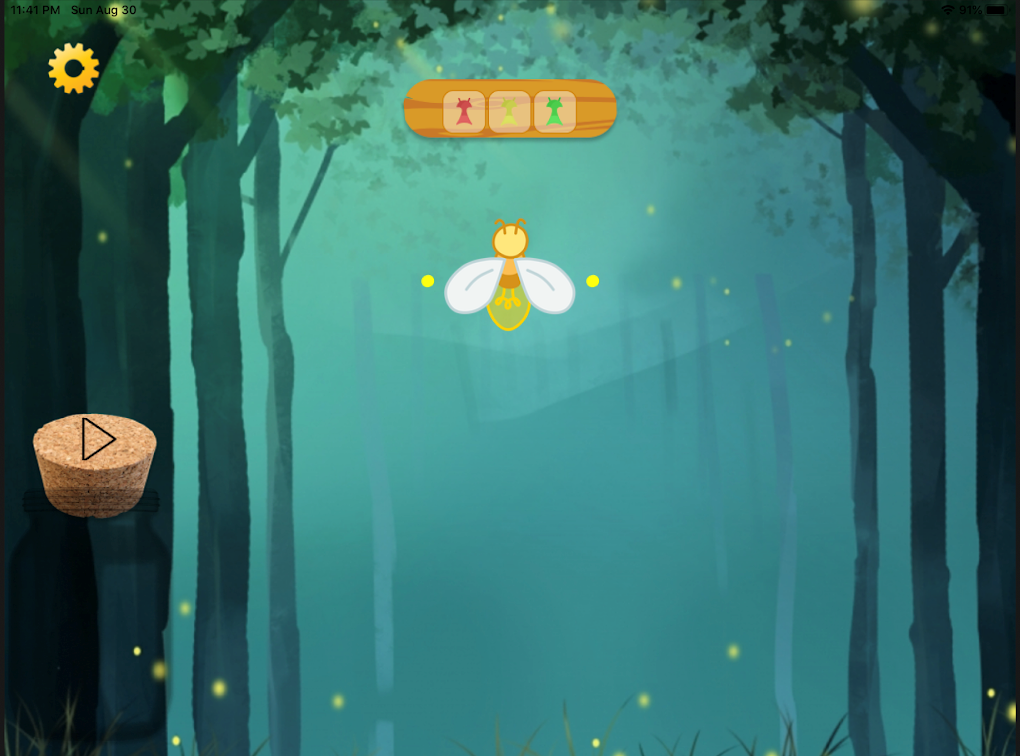
\includegraphics[width=10cm]{figures/newScreenFlows/newbody.png}
    \caption{Body popup}
    \label{fig:newbody}
\end{figure}

When the child taps the body part, they can choose from three different colors that represent different tempos.

\subsection{Firefly Right Wing Selection}

\begin{figure}[H]
    \centering
    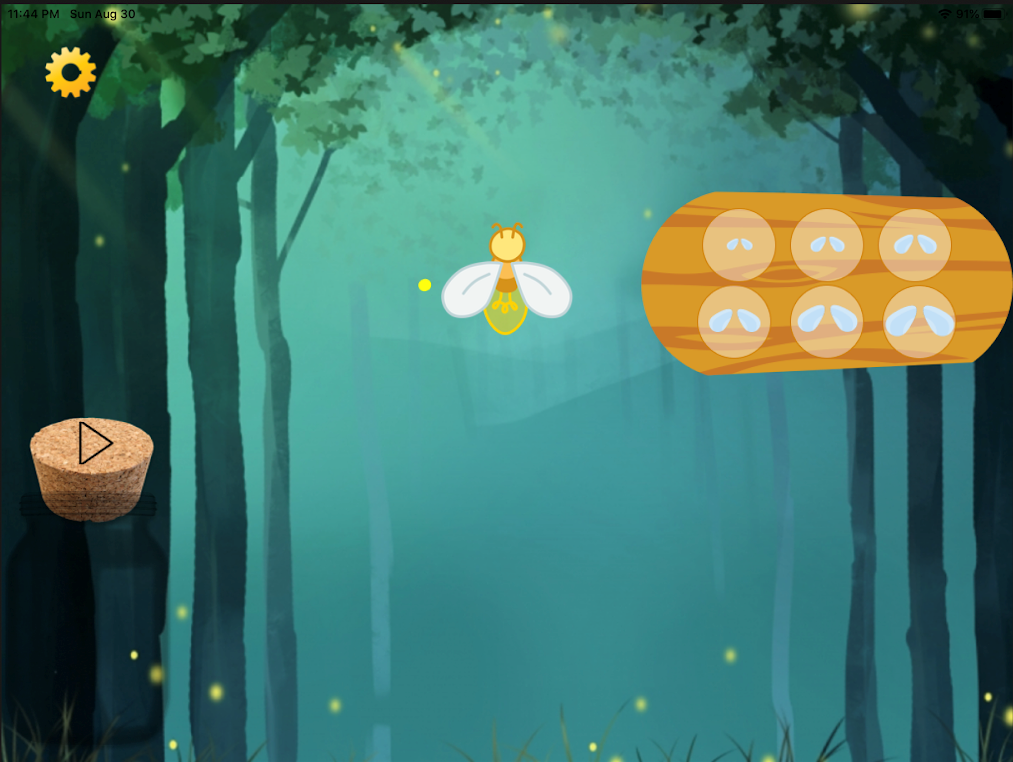
\includegraphics[width=10cm]{figures/newScreenFlows/newrightwing.png}
    \caption{Right Wing popup}
    \label{fig:newrightwing}
\end{figure}

When the child taps the right wing, they will be able to choose how many times the firefly will play the pattern.

\subsection{Firefly Left Wing Selection}

\begin{figure}[H]
    \centering
    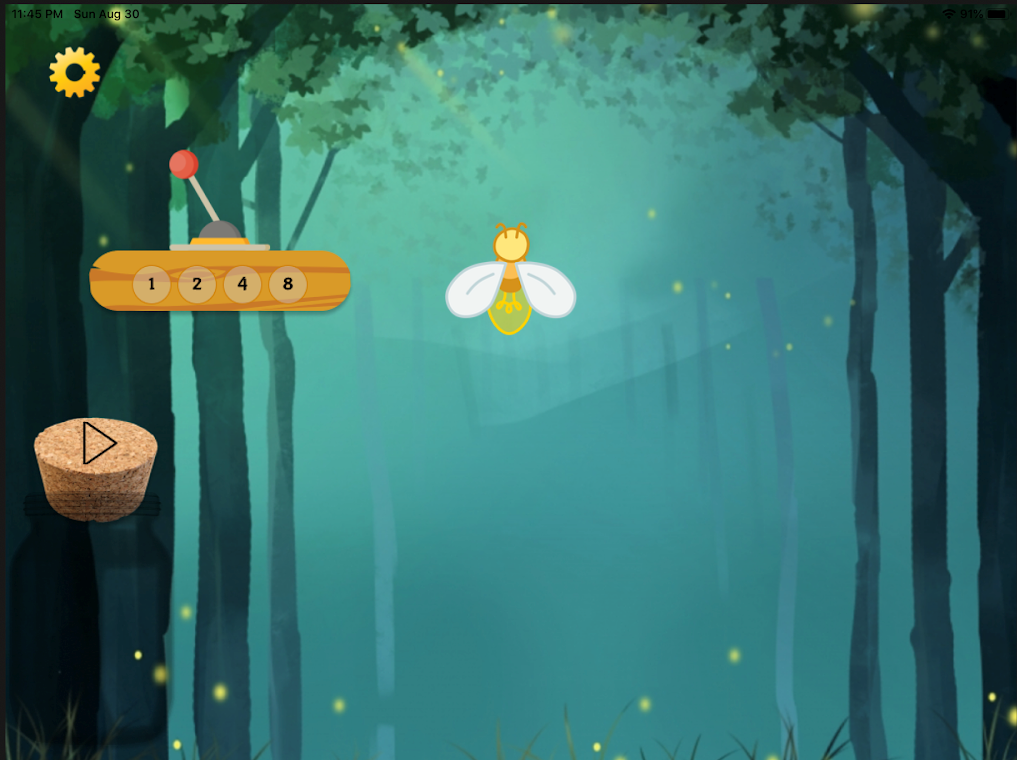
\includegraphics[width=10cm]{figures/newScreenFlows/newleftwing2.png}
    \caption{Left wing popup notes}
    \label{fig:newleftwing}
\end{figure}

When the child taps the left wing, they will be able to choose the first note to play.

\begin{figure}[H]
    \centering
    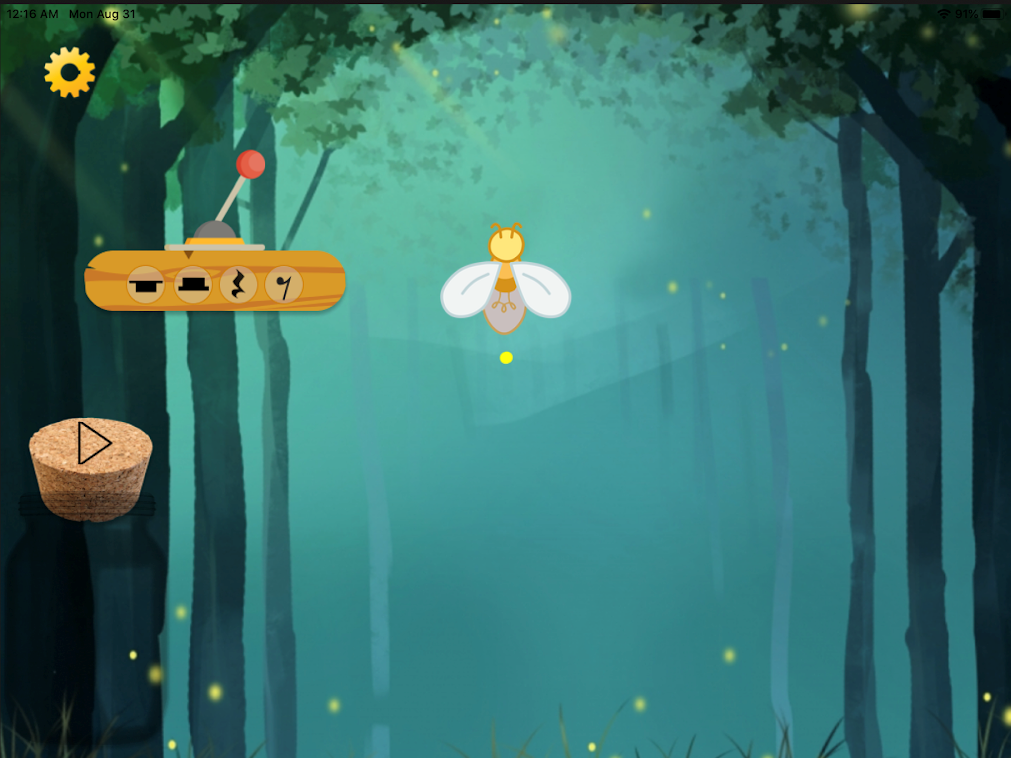
\includegraphics[width=10cm]{figures/newScreenFlows/newleftwing.png}
    \caption{Left wing popup rests}
    \label{fig:newleftwing2}
\end{figure}

The lever can be toggled to show the rests.

\subsection{Firefly Tail Selection}

\begin{figure}[H]
    \centering
    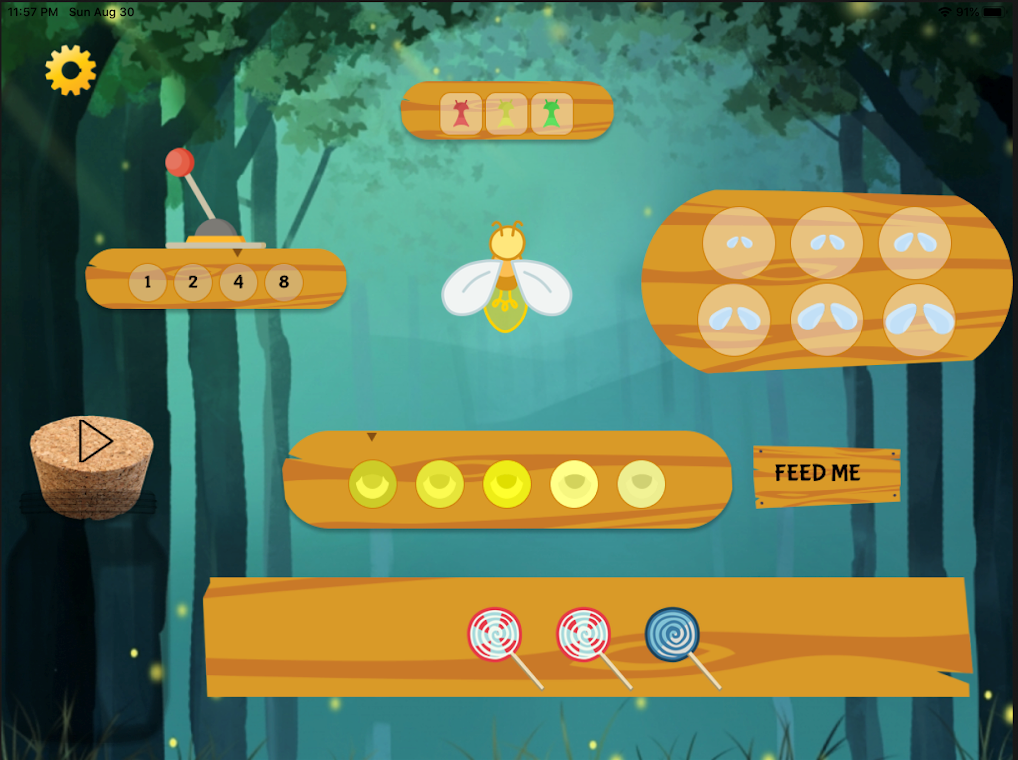
\includegraphics[width=10cm]{figures/newScreenFlows/candypreview.png}
    \caption{Tail popup}
    \label{fig:newtail}
\end{figure}

When the child taps the tail, they will be able to choose the patterns based on their first note. The child will be able to see the preview of the candy patterns.

\subsection{Feed Me}

\begin{figure}[H]
    \centering
    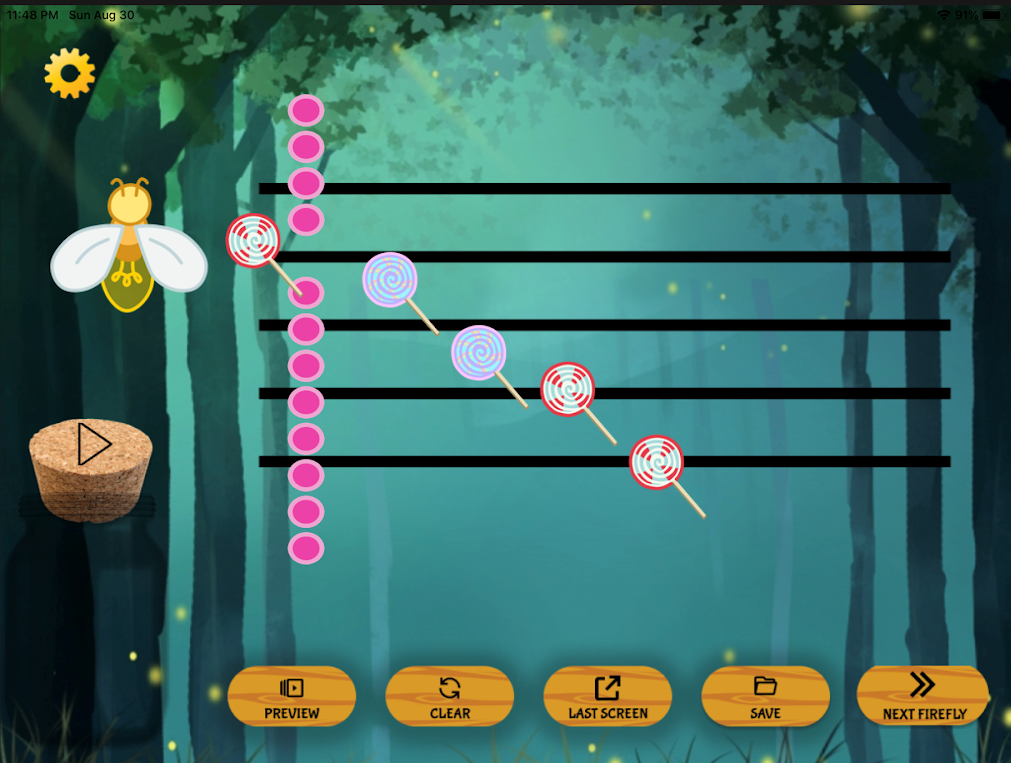
\includegraphics[width=10cm]{figures/newScreenFlows/newfeedme.png}
    \caption{Left wing popup notes}
    \label{fig:newleftwing}
\end{figure}

After choosing the pattern, the child can tap the feed me button which brings up the staff where they can place the candies to give the firefly pitches. In this screen, there is also a preview button which plays the current firefly to see how it will sound like. The clear button resets the candy placements. The last screen button allows you to go back to editing the firefly. The save buttons saves the current firefly configuration. The next firefly button will go to the next editable firefly.

\subsection{Jar Play}



\subsection{Menu Settings}

\begin{figure}[H]
    \centering
    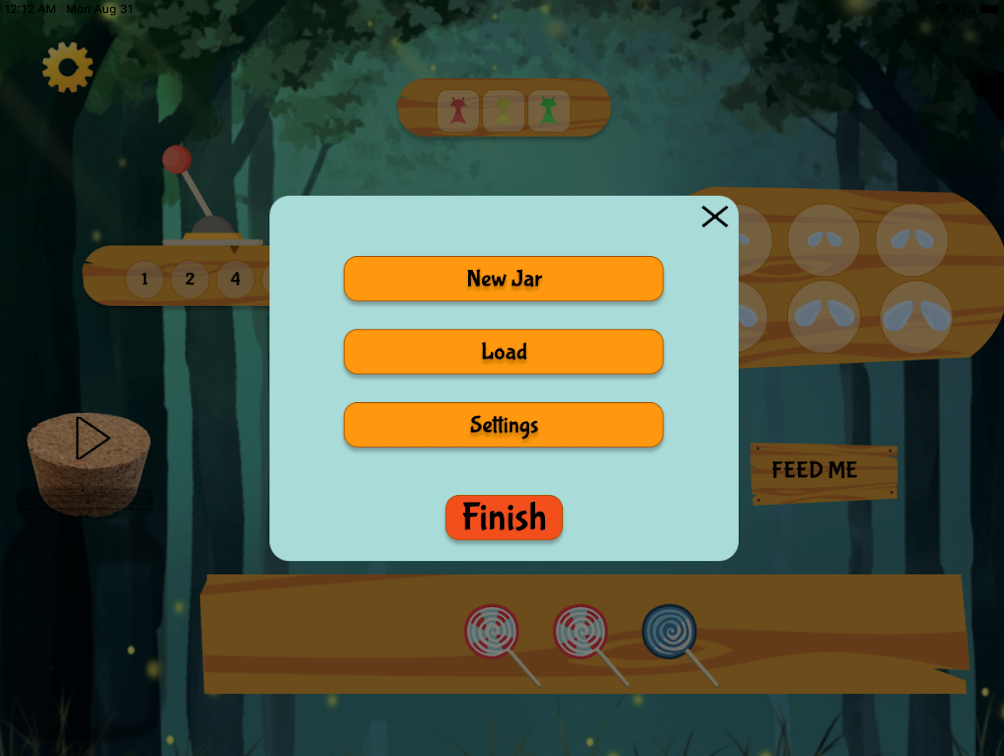
\includegraphics[width=10cm]{figures/newScreenFlows/newmainsettings.png}
    \caption{Settings}
    \label{fig:newsettings}
\end{figure}

When the child taps on the gear icon, this will bring up a popup menu where can tap three different buttons. The new jar button will create a new jar of fireflies. The load button will allow him to load previously saved jars. The settings button will allow him to change some preferences.

\subsection{Visual Settings}

\begin{figure}[H]
    \centering
    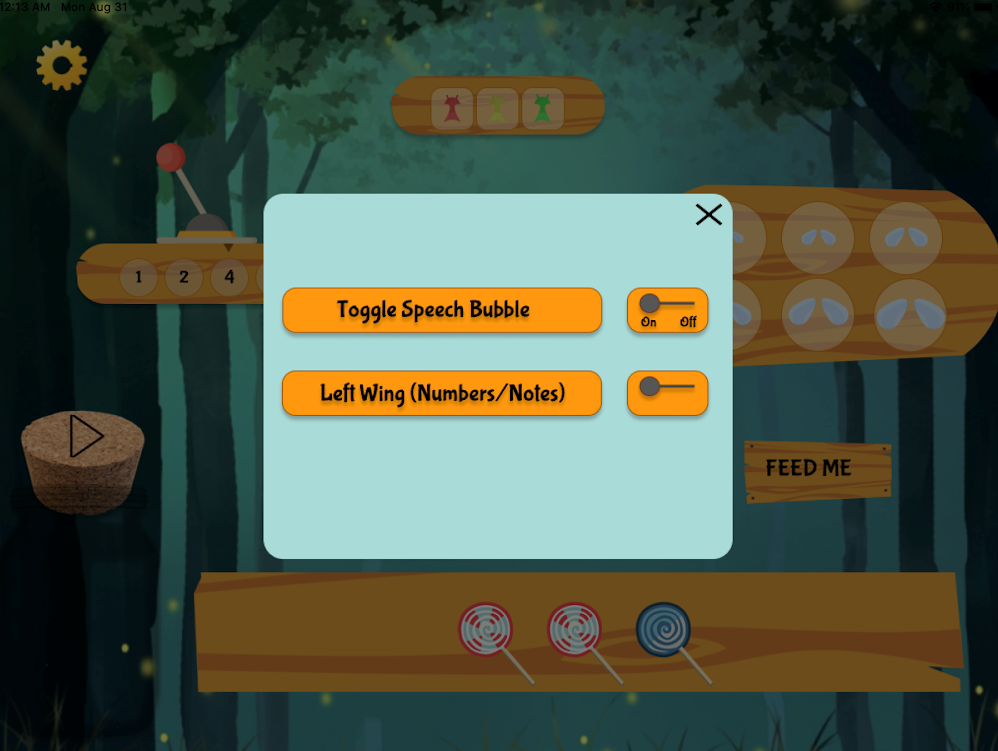
\includegraphics[width=10cm]{figures/newScreenFlows/newsettings.png}
    \caption{Visual settings}
    \label{fig:newvisettings}
\end{figure}

After tapping the settings button, the child may toggle the speech bubble guide and toggle to use numbers or notes for the left wing.

\subsection{Load Screen}

\begin{figure}[H]
    \centering
    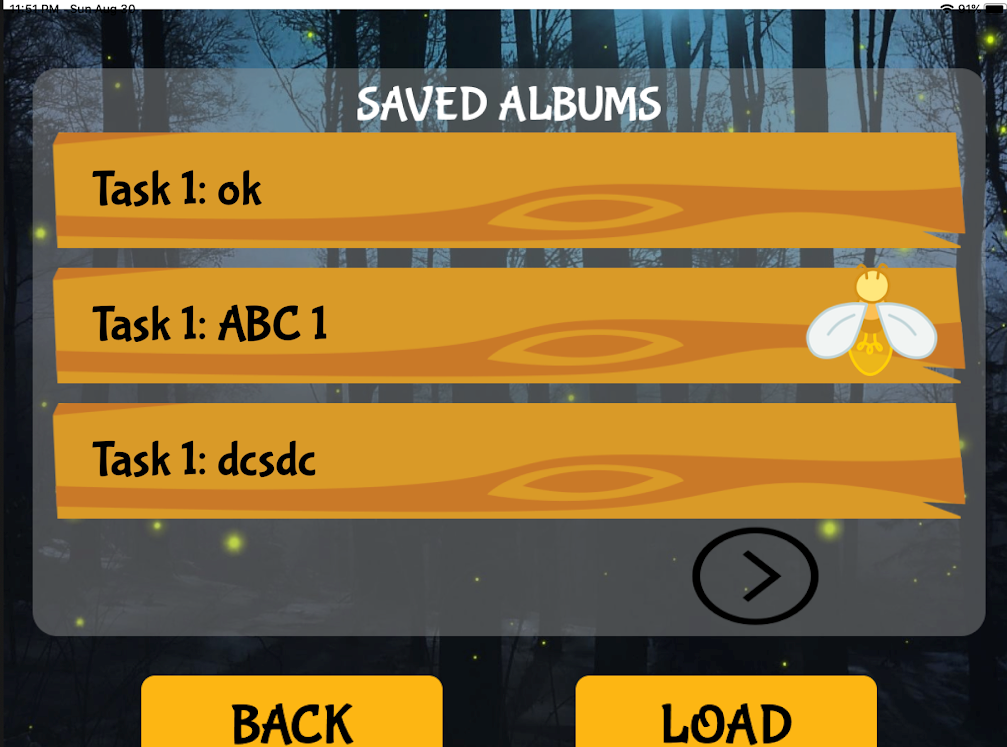
\includegraphics[width=10cm]{figures/newScreenFlows/newload.png}
    \caption{Load screen}
    \label{fig:newload}
\end{figure}
After tapping the load button, this brings up the previous jars that the child made and can load from his previous saves.

% \section{Use Case Diagram}
% \begin{figure}[!htb]
%     \centering
%     \includegraphics{figures/UseCaseDiagram.PNG}
%     \caption{Use Case Diagram of Firefly}
%     \label{fig:my_label}
% \end{figure}

% This is the use case diagram of Firefly. These are all the actions that the user is allowed to do within the application.

\section{Deployment Plan}
FireflyX will be developed using Xcode using the Swift language. The application once compiled can be uploaded to the Apple App Store where anyone may download the application for free. We will then use TestFlight to distribute our application. This is because Testflight allows for remote testing. To use TestFlight, we will upload beta builds of FireflyX, and invite testers using their email addresses. Testers will then check their email to accept the invitation to test the application. In order for the testers to install FireflyX, They will have to use the TestFlight application in their iPad after accepting the invitation in their email.

The files will then be saved locally this includes the songs and their respective jars, these files will be exportable with the use of the JSON. Using the JSON another user in a different iPad can retrieve the same environment by loading the JSON sent. This will be done since the application is also connected to Google's Firebase storage to save the data online in JSON format. A diagram showing the deployment plan is shown in figure \ref{deploymentPlan}.

\begin{figure}[H]
    \centering
    \includegraphics[width=15cm]{figures/deploymentPlan.png}
    \caption{FireflyX deployment plan}
    \label{deploymentPlan}
\end{figure}